\section{VECTORS AND MATRICES}
\subsection{Vectors in $\mathbb{R}^n$}

\begin{exercise} \label{e1.1.1}
    Given \( \mathbf{x} = \begin{bmatrix} 2 \\ 3 \end{bmatrix} \) and \( \mathbf{y} = \begin{bmatrix} -1 \\ 1 \end{bmatrix} \) calculate the following both algebraically and geometrically.
    \begin{enumerate}
        \item \( \mathbf{x}+\mathbf{y} \)
        \item \( \mathbf{x}-\mathbf{y} \)
        \item \( \mathbf{x}+2\mathbf{y} \)
        \item \( \frac{1}{2}\mathbf{x}+\frac{1}{2}\mathbf{y} \)
        \item \( \mathbf{y}-\mathbf{x} \)
        \item \( 2\mathbf{x}-\mathbf{y} \)
        \item \( \left\lVert \mathbf{x} \right\rVert \)
        \item \( \frac{\mathbf{x}}{\left\lVert \mathbf{x} \right\rVert} \)
    \end{enumerate}
    
    \begin{proof}
        \begin{enumerate}
            \item \( \mathbf{x}+\mathbf{y}=\begin{bmatrix} 2 \\ 3 \end{bmatrix} + \begin{bmatrix} -1 \\ 1 \end{bmatrix} = \begin{bmatrix} 2+(-1) \\ 3 + 1 \end{bmatrix} = \begin{bmatrix} 1 \\ 4 \end{bmatrix} \)
        \end{enumerate}
        
        The idea is similar for the rest.
    \end{proof}
\end{exercise}

\begin{exercise} \label{e1.1.2}
    Three vertices of a parallelogram are \( \begin{bmatrix} 1 \\ 2 \\ 1 \end{bmatrix}, \begin{bmatrix} 2 \\ 4 \\ 3 \end{bmatrix},\text{ and } \begin{bmatrix} 3 \\ 1 \\ 5 \end{bmatrix} \). What are all the possible positions of the fourth vertex? Give your reasoning.
    
    \begin{proof}
        The three vertices given already define a plane, which implies that any fourth vertex would have to belong to the plane as well. Thus the problem is reduced to finding the three points in the plane that will produce a parallelogram. Each solution is given by the sum of the three original vectors where one of them is negative. The three points then are given by:
        \begin{align*}
            \begin{bmatrix} 1 \\ 2 \\ 1 \end{bmatrix} + \begin{bmatrix} 2 \\ 4 \\ 3 \end{bmatrix} - \begin{bmatrix} 3 \\ 1 \\ 5  \end{bmatrix} &= \begin{bmatrix} 0 \\ 5 \\ -1 \end{bmatrix} \\
            \begin{bmatrix} 2 \\ 4 \\ 3 \end{bmatrix} + \begin{bmatrix} 3 \\ 1 \\ 5 \end{bmatrix} - \begin{bmatrix} 1 \\ 2 \\ 1 \end{bmatrix} &= \begin{bmatrix} 4 \\ 3 \\ 7 \end{bmatrix} \\
            \begin{bmatrix} 3 \\ 1 \\ 5 \end{bmatrix} + \begin{bmatrix} 1 \\ 2 \\ 1 \end{bmatrix} - \begin{bmatrix} 2 \\ 4 \\ 3 \end{bmatrix} &= \begin{bmatrix} 2 \\ -1 \\ 3 \end{bmatrix} \\
        \end{align*}
        
        \begin{center}
            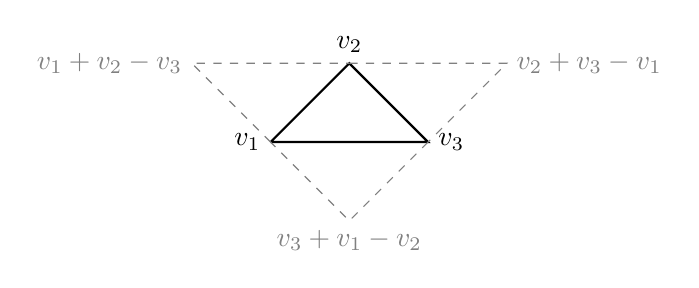
\begin{tikzpicture}
                \draw[thick] (-1,0) node[anchor=east] {$v_1$}
                -- (0,1) node[anchor=south] {$v_2$}
                -- (1,0) node[anchor=west] {$v_3$}
                -- (-1,0);
                
                \draw[color=gray,dashed] (0,1)
                -- (2,1) node[anchor=west] {$v_2+v_3-v_1$}
                -- (1,0);
                
                \draw[color=gray,dashed] (1,0)
                -- (0,-1) node[anchor=north] {$v_3+v_1-v_2$}
                -- (-1,0);
                
                \draw[color=gray,dashed] (-1,0)
                -- (-2,1) node[anchor=east] {$v_1+v_2-v_3$}
                -- (0,1);
            \end{tikzpicture}
        \end{center}
    \end{proof}
\end{exercise}

\begin{exercise} \label{e1.1.3}
    The origin is at the center of a regular polygon.
    \begin{enumerate}
        \item What is the sum of the vectors to each of the vertices of the polygon? Give your reasoning.
        \item What is the sum of the vectors from one fixed vertex to each of the remaining vertices? Give your reasoning
    \end{enumerate}
    
    \begin{proof}
        \begin{enumerate}
            \item Let one of the vertices of the polygon be at \( (r,0) \), where \(r>0\). By symmetry of the polygon, it follows that the sum of all the \(y\)-components of the vectors is \( 0 \). One can use the identity
            \[
            \sum_{k=0}^{n-1} \cos(a+kd) = \cos\left( \frac{a+(n-1)d}{2} \right)\frac{ \sin\left( n \frac{d}{2} \right) }{\sin\left( \frac{d}{2} \right)}
            \]
            to show that the \(x\)-components of the vectors sum to \( 0 \). Thus the sum of the vectors is \( \mathbf{0} \).
            
            \item Let \( v_i \) denote the vector from the origin to the \( i^{th} \) vertex, where the vector from the center to the source vertex is \( v_1 \). Let \( w_i \) denote the vector from the source vertex to the \( i^{th} \) vertex. Then \( w_i = v_i - v_1 \). Thus
            
            \begin{align*}
                \sum_{i=2}^n w_i &= \sum_{i=2}^n (v_i - v_1) \\
                &= \sum_{i=2}^n v_i - (n-1)v_1 \\
                \intertext{and by the previous problem}
                &= -nv_1
            \end{align*}
        \end{enumerate}
    \end{proof}
\end{exercise}

\begin{exercise} \label{e1.1.4}
    Given \( \triangle ABC \), let \( M \) and \( N \) denote the midpoints of \( \overline{AB} \) and \( \overline{AC} \), respectively. Prove that \( \overrightarrow{MN} = \frac{1}{2} \overrightarrow{BC} \).
    
    \begin{proof}
        Set \( A = (0,0) \). Then
            \begin{align*}
                \overrightarrow{M} &= \frac{1}{2}\overrightarrow{AB} \\
                \overrightarrow{N} &= \frac{1}{2}\overrightarrow{AC} \\
                \intertext{So that}
                \overrightarrow{MN} &= \overrightarrow{M}-\overrightarrow{N} \\
                &= \frac{1}{2}\overrightarrow{AB} - \frac{1}{2}\overrightarrow{AC} \\
                &= \frac{1}{2} \left( \overrightarrow{AB}-\overrightarrow{AC} \right) \\
                &= \frac{1}{2} \overrightarrow{BC}
            \end{align*}
            \begin{center}
                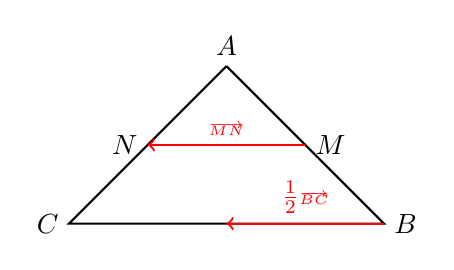
\begin{tikzpicture}
                    \draw[thick] (0,1) node[anchor=south] {$A$}
                    --(1,0) node[anchor=west] {$M$}
                    --(2,-1) node[anchor=west] {$B$}
                    --(-2,-1) node[anchor=east] {$C$}
                    --(-1,0) node[anchor=east] {$N$}
                    --(0,1);
                    
                    \draw[red,thick,->] (1,0) -- (-1,0);
                    \draw[red] (0,0) node[anchor=south] {$\tiny{\overrightarrow{MN}}$};
                    
                    \draw[red,thick,->] (2,-1) -- (0,-1);
                    \draw[red] (1,-1) node[anchor=south] {$\tiny{\frac{1}{2}\overrightarrow{BC}}$};
                \end{tikzpicture}
            \end{center}
    \end{proof}
\end{exercise}

\begin{exercise} \label{e1.1.5}
    Let \( ABCD \) be an arbitrary quadrilateral. Let \( P,Q,R,\text{ and } S \) be the midpoints of \( \overline{AB},\overline{BC},\overline{CD},\text{ and } \overrightarrow{DA} \), respectively. Use vector methods to prove that \( PQRS \) is a parallelogram.
    
    \begin{proof}
        By the previous exercise, we know that
        \begin{alignat*}{3}
            \overrightarrow{SP} &= \frac{1}{2}\overrightarrow{DB} &= \overrightarrow{RQ}  \\
            \overrightarrow{PQ} &= \frac{1}{2}\overrightarrow{AC} &= \overrightarrow{SR} 
        \end{alignat*}
        implying that \( PQRS \) is a parallelgram.
        
        \begin{center}
            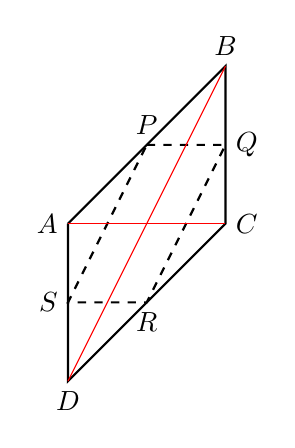
\begin{tikzpicture}
                \draw[thick] (0,0) node[anchor=east] {$A$}
                -- (1,1) node[anchor=south] {$P$}
                -- (2,2) node[anchor=south] {$B$}
                -- (2,1) node[anchor=west] {$Q$}
                --(2,0) node[anchor=west] {$C$}
                --(1,-1) node[anchor=north] {$R$}
                --(0,-2) node[anchor=north] {$D$}
                --(0,-1) node[anchor=east] {$S$}
                --(0,0);
                
                \draw[dashed,thick] (1,1)
                --(2,1)
                --(1,-1)
                --(0,-1)
                --(1,1);
                
                \draw[red] (0,-2)
                --(2,2);
                
                \draw[red] (0,0)
                --(2,0);
            \end{tikzpicture}
        \end{center}
    \end{proof}
\end{exercise}


\subsection{Dot Product}

\begin{exercise} \label{e1.2.1}
    For each of the following pairs of vectors \( x \) and \( y \), calculate \( x \cdot y \) and the angle \( \theta \) between the vectors.
    \[
    x=\begin{bmatrix}2\\5\end{bmatrix},y=\begin{bmatrix}-5\\2\end{bmatrix}
    \]
    \begin{proof}
        \[ x \cdot y = 2(-5)+5(2) = 0 \]
        and
        \[
        \theta = \cos^{-1}{\frac{x\cdot y}{\lVert x \rVert \lVert y \rVert}} = \frac{\pi}{2}
        \]
        The rest of the problems are similar.
    \end{proof}
\end{exercise} %1.2.1

\begin{exercise} \label{e1.2.2}
    For each pair of vectors in Exercise 1, calculate \( \text{proj}_{y}x \) and \( \text{proj}_{x}y \)
    
    \begin{proof}
        Since we saw that \( x \cdot y = 0 \), we have
        \[ \text{proj}_{x}y = \frac{x \cdot y}{\lVert x \rVert^2}x = \text{proj}_{y}x = \frac{x \cdot y}{\lVert y \rVert^2}y = 0 \]
        The remaining are similar.
    \end{proof}
\end{exercise} %e1.2.2

\begin{exercise} \label{e1.2.3}
    Find the angle between the long diagonal of a cube and a face diagonal.
    
    \begin{proof}
        Wlog, take the unit cube. Denote the long diagonal \( l = \begin{bmatrix} 1\\1\\1 \end{bmatrix} \) and, wlog, the short diagonal \( s = \begin{bmatrix} 0 \\ 1 \\ 1 \end{bmatrix} \). Then
        \[
        \theta = \cos^{-1}\frac{l \cdot s}{\lVert l \rVert \lVert s \rVert} = \frac{2}{\sqrt{3}\sqrt{2}} = \sqrt{\frac{2}{3}}
        \]
    \end{proof}
\end{exercise} %e1.2.3

\begin{exercise} \label{1.2.4}
    Find the angle that the long diagonal of a \( 3 \times 4 \times 5 \) rectangular box makes with the longest edge.
    
    \begin{proof}
        
    \end{proof}
\end{exercise} %e1.2.4

\begin{exercise} \label{e1.2.5}
    Suppose \( x, y \in \mathbb{R}^n \), \( \lVert x \rVert =2, \lVert y \rVert =1 \), and the angle \( \theta \) between \( x \) and \( y \) is \( \theta = \arccos{\frac{1}{4}} \). Prove that the vectors \( x-3y \) and \( x+y \) are orthogonal.

    \begin{proof}
        Since \( \theta = \arccos{\frac{1}{4}} \) it follows that
        \begin{align*}
        \frac{1}{4} = &\cos{\theta} = \frac{x \cdot y}{\lVert x \rVert \lVert y \rVert} \\
        \frac{1}{2} &= x \cdot y
        \end{align*}
        Thus
        \begin{align*}
            (x-3y) \cdot (x+y) &= (x \cdot x) + (x \cdot y) - 3(y \cdot x) + (y \cdot y)\\
            &= 4 - 2 (x \cdot y) -3 \\
            &= 0
        \end{align*}
    \end{proof}
\end{exercise} %e1.2.5

\begin{exercise} \label{e1.2.6}
    Suppose \( x,y,z \in \mathbb{R}^2 \) are unit vectors satisfying \( x+y+z=0 \). What can you say about the angles between each pair?
    
    \begin{proof}
        Note that, more generally, we have
        \[ \lVert x_1 \rVert = \lVert x_2 \rVert = \lVert x_3 \rVert = 1 \]
        and
        \[ x_3 = -x_1-x_2 \]
        Thus
        \begin{align*}
             0 &= (x_1+x_2+x_3) \cdot (x_1+x_2+x_3) \\
             &= 3 + 2\left((x_1 \cdot x_2) + (x_1 \cdot x_3) + (x_2 \cdot x_3)\right) \\
             &= 3 + 2\left( (x_1 \cdot x_2) + (x_1 \cdot (-x_1-x_2)) + (x_2 \cdot (-x_1-x_2)) \right) \\
             &= 3 + 2\left( (x_1 \cdot x_2) - 2 - 2(x_1 \cdot x_2) \right) \\
             &= 3 - 4 - 2(x_1 \cdot x_2) \\
             &= -1 - 2(x_1 \cdot x_2)
             \intertext{thus}
             -\frac{1}{2} &= x_1 \cdot x_2
        \end{align*}
        
        It therefore follows that the angle, \( \theta \), between any pair is given by
        \[ \theta = \arccos{-\frac{1}{2}} = \frac{2\pi}{3} \]
    \end{proof}
\end{exercise} %e1.2.6

\begin{exercise} \label{e1.2.7}
    Let \( e_1 = \begin{bmatrix} 1 \\ 0 \\ 0  \end{bmatrix} \), \( e_2 = \begin{bmatrix} 0 \\ 1 \\ 0  \end{bmatrix} \), and \( e_3 = \begin{bmatrix} 0 \\ 0 \\ 1  \end{bmatrix} \) be the so-called \emph{standard basis vectors} of \( \mathbb{R}^3 \). Let \( x \in \mathbb{R}^3 \) be a nonzero vetor. For \( i = 1,2,3 \), let \( \theta_i \) denote the angle between \( x \) and \( e_i \). Compute \( \cos^2{\theta_1} + \cos^2{\theta_2} + \cos^2{\theta_3} \).
    
    \begin{proof}
        Let \( x = \begin{bmatrix} x_1 \\ x_2 \\ x_3 \end{bmatrix} \neq \begin{bmatrix} 0 \\ 0 \\ 0 \end{bmatrix} \). Then
        \begin{align*}
            \cos^2{\theta_1}+\cos^2{\theta_2}+\cos^2{\theta_3} &= \frac{\sum_{i=1}^n (x_i \cdot e_i)^2}{\lVert x \rVert^2} \\
            &= \frac{\sum_{i=1}^n x_i^2}{\sum_{i=1}^n x_i^2} \\
            &= 1
        \end{align*}
    \end{proof}
\end{exercise} %e1.2.7

\begin{exercise} \label{e1.2.8}
    Let \( x = \begin{bmatrix} 1 \\ 1 \\ 1 \\ \vdots \\ 1 \end{bmatrix} \) and \( y = \begin{bmatrix} 1 \\ 2 \\ 3 \\ \vdots \\ n \end{bmatrix} \in \mathbb{R}^n \). Let \( \theta_n \) be the angle between \( x \) and \( y \). Find \( \displaystyle \lim_{n \rightarrow \infty} \theta_n \).
    
    \begin{proof}
        Note that
        \[
        \theta_n = \arccos{\frac{x \cdot y}{\lVert x \rVert \lVert y \rVert}} 
        \]
        We observe that
        \begin{align*}
            \frac{x \cdot y}{\lVert x \rVert \lVert y \rVert} &= \frac{\sum_{i=1}^n i}{\sqrt{n}\sqrt{\sum_{i=1}^n i^2}} \\
            &= \left( \frac{n(n+1)}{2} \right) \left( \frac{\sqrt{6}}{n\sqrt{n+1}\sqrt{2n+1}} \right) \\
            &= \frac{1}{2} \left( \sqrt{\frac{6n+6}{2n+1}} \right)
        \end{align*}
        and therefore
        \begin{align*}
            \lim_{n \rightarrow \infty} \frac{x \cdot y}{\lVert x \rVert \lVert y \rVert} &= \lim_{n \rightarrow \infty} \frac{1}{2} \left( \sqrt{\frac{6n+6}{2n+1}} \right) \\
            &= \frac{\sqrt{3}}{2}
        \end{align*}
        Thus, by continuity of \( \arccos \), we have
        \begin{align*}
            \lim_{n \rightarrow \infty} \theta_n &= \lim_{n \rightarrow \infty} \arccos{\frac{1}{2} \left( \sqrt{\frac{6n+6}{2n+1}} \right)} \\
            &= \arccos{\frac{\sqrt{3}}{2}} \\
            &= \frac{\pi}{6}
        \end{align*}
    \end{proof}
\end{exercise} %e1.2.8


\begin{exercise} \label{e1.2.9}
    With regard to the proof of Proposition 2.3, how is \( t_0y \) related to \( x^{\vert \vert} \)? What does this say about \( \text{proj}_y x \)?
    
    \begin{proof}
        Note that
        \[ x^{\vert \vert} = \frac{x \cdot y}{\lVert y \rVert^2} y = \text{proj}_y x = -t_0y\]
        
        Intuitively, this simply means that the function \( g \), presented in the proof of Proposition 2.3, is minimized when the only non-zero component of \( x + ty \) is \( x^{\perp} \). That is
        
        \begin{align*}
            \lVert x+t_0y \rVert^2 &= \lVert x^{\vert\vert}+x^{\perp}+t_0y \rVert^2 \\
            &= \lVert x^{\perp} \rVert^2
        \end{align*}
    \end{proof}
\end{exercise} %e1.2.9

\begin{exercise} \label{e1.2.10}
    Use vector methods to prove that a parallelogram is a rectangle iff its diagonals have the same length.
    
    \begin{proof}
        Note that if \( u, v \neq 0 \), then 
        \begin{align*}
            \lVert v+u \rVert^2 &= \lVert v-u \rVert^2 \\
            (v+u) \cdot (v+u) &= (v-u) \cdot (v-u) \\
            v \cdot v + 2 v\cdot u + u \cdot u &= v \cdot v - 2 v \cdot u + u \cdot u \\
            &\text{iff} \\
            v \cdot u &= 0
        \end{align*}
        
        \begin{center}
            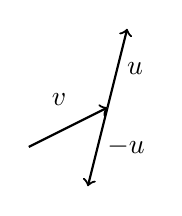
\begin{tikzpicture}
                \draw[->,thick] (0,0)--(1,0.5);
                \draw (0.6,0.6) node[anchor=east] {$v$};
                \draw[->,thick] (1,0.5)--(1.25,1.5);
                \draw (1.125,1) node[anchor=west] {$u$};
                \draw[->,thick] (1,0.5)--(0.75,-0.5);
                \draw (0.875,0) node[anchor=west] {$-u$};
            \end{tikzpicture}
        \end{center}
        
        Thus, if ABCD is a parallelogram with diagonals \( D_1, D_2 \neq 0 \), then
        \begin{align*} \lVert D_1 \rVert^2 = \lVert \overrightarrow{AD} + \overrightarrow{DC} \rVert^2 = &\lVert \overrightarrow{BC} + \overrightarrow{CD} \rVert^2 = \lVert \overrightarrow{AD} - \overrightarrow{DC} \rVert^2 = \lVert D_2 \rVert^2 \\
        &\text{iff} \\
        \overrightarrow{AD} \cdot \overrightarrow{DC} &= 0
        \end{align*}
        which implies the result.
    \end{proof}
\end{exercise} %e1.2.10

\begin{exercise} \label{e1.2.11}
    Use the fundamental properties of the dot product to prove that
    \[ \lVert x+y \rVert^2 + \lVert x-y \rVert^2 = 2\left( \lVert x \rVert^2 + \lVert y \rVert^2 \right)  \]
    
    \begin{proof}
        \begin{align*}
            \lVert x+y \rVert^2 + \lVert x-y \rVert^2 &= (x+y) \cdot (x+y) + (x-y) \cdot (x-y) \\
            &= (x \cdot x) + 2(x \cdot y) + (y \cdot y) + (x \cdot x) - 2(x \cdot y) + (y \cdot y) \\
            &= 2(x \cdot x) + 2 (y \cdot y) \\
            &= 2 \left( \lVert x \rVert^2 + \lVert y \rVert^2 \right)
        \end{align*}
    \end{proof}
\end{exercise} %e1.2.11

\begin{exercise} \label{e1.2.12}
    Use the dot product to prove the law of cosines
    
    \[ c^2 = a^2 + b^2 -2ab\cos{\theta} \]
    
    \begin{center}
        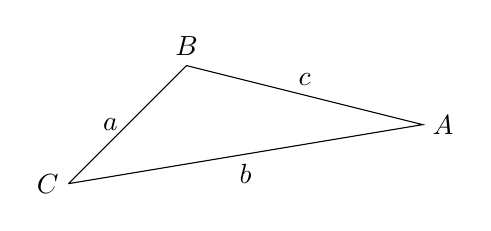
\begin{tikzpicture}
            \draw[] (0,0)
            --(0.75,0.75) node[anchor=east] {$a$}
            --(1.5,1.5) node[anchor=south] {$B$}
            --(3,1.125) node[anchor=south] {$c$}
            --(4.5,0.75) node[anchor=west] {$A$}
            --(2.25,0.375) node[anchor=north] {$b$}
            --(0,0) node[anchor=east] {$C$};
        \end{tikzpicture}
    \end{center}
    
    \begin{proof}
        \begin{align*}
            c^2 &= \lVert \overrightarrow{CA} - \overrightarrow{CB} \rVert^2 \\
            &= (\overrightarrow{CA}-\overrightarrow{CB}) \cdot (\overrightarrow{CA}-\overrightarrow{CB}) \\
            &= \lVert \overrightarrow{CA} \rVert^2 + \lVert \overrightarrow{CB} \rVert^2 - 2\left( \overrightarrow{CA} \cdot \overrightarrow{CB} \right) \\
            &= a^2 + b^2 - 2ab\cos{\theta}
        \end{align*}
    \end{proof}
\end{exercise} %e1.2.12

\begin{exercise} \label{e1.2.13}
    Use vector methods to prove that the diagonals of a parallelogram are orthogonal if and only if the parallelogram is a rhombus (i.e., has all sides of equal length).
    
    \begin{proof}Consider the parallelogram
    
        \begin{center}
            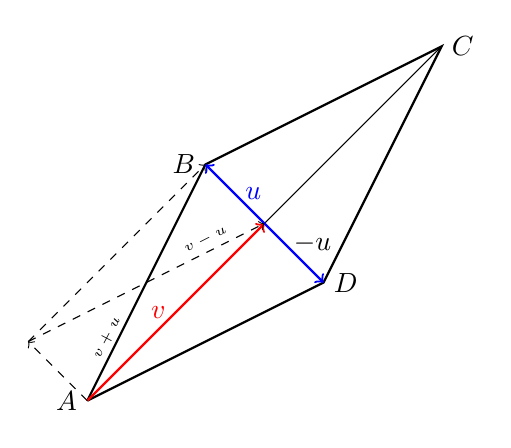
\begin{tikzpicture}
                \draw[thick] (0,0)
                -- (1.5,3) node[anchor=east] {$B$}
                -- (4.5,4.5) node[anchor=west] {$C$}
                -- (3,1.5) node[anchor=west] {$D$}
                -- (0,0) node[anchor=east] {$A$};
                
                \draw (0,0) -- (4.5,4.5);
                \draw (1.5,3) -- (3,1.5);
                
                \draw[->,thick,red] (0,0) 
                -- (1.125,1.125) node[anchor=east] {$v$}
                -- (2.25,2.25);
                
                \draw[->,thick,blue] (2.25,2.25)
                -- (1.875,2.625) node[anchor=west] {$u$}
                -- (1.5,3);
                
                \draw[->,thick,blue] (2.25,2.25)
                -- (2.625,1.875)
                -- (3,1.5);
                
                \draw (2.5,2) node[anchor=west] {$-u$};
                
                \draw[->, dashed] (0,0)
                -- (-0.75,0.75);
                
                \draw[->, dashed] (-0.75,0.75)
                -- (1.5,3);
                
                \draw[->, dashed] (-0.75,0.75)
                -- (2.25,2.25);
                
                \node[rotate=62] at (0.25,0.8) {\tiny{$v+u$}};
                \node[rotate=27] at (1.5,2.05) {\tiny{$v-u$}};
            \end{tikzpicture}
        \end{center}
        
        From Exercise \ref{e1.2.10},
        
        \[ \lVert v+u \rVert = \lVert v-u \rVert \text{ iff } v \cdot u = 0 \]
    \end{proof}
\end{exercise} %e1.2.13

\begin{exercise} \label{e1.2.14}
    Use vector methods to prove that a triangle inscribed in a circle and having a diameter as one of the sides must be a right triangle.
    
    \vspace{1cm}
    
    \emph{Geometric Challenge:} More generally, given two points \( A \) and \( B \) in the plane, what is the locus of points \( X \) so that \( \angle AXB \) has a fixed measure?
    
    \begin{proof}
        Note that this is a simple consequence of the inscribed angle theorem. Using vector methods, given
        
        \begin{center}
            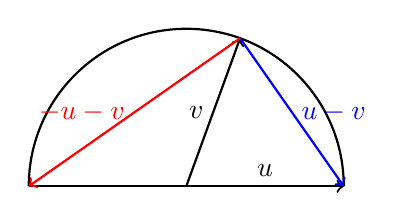
\begin{tikzpicture}
                \draw[thick] (2,0) arc (0:180:2);
                \draw[thick] (-2,0) -- (0,0);
                \draw[thick,->] (0,0) -- (0.684040287,1.879385242);
                \draw[thick,->] (0,0) -- (2,0);
                \draw[->,color=blue,thick] (0.684040287,1.879385242) -- (2,0);
                \draw[->,color=red,thick] (0.684040287,1.879385242) -- (-2,0);
                
                \draw (0.342020143,0.939692621) node[anchor=east] {$v$};
                \draw (1,0) node[anchor=south] {$u$};
                
                \draw[color=blue] (1.342020144,0.939692621) node[anchor=west] {$u-v$};
                \draw[color=red] (-0.657979856,0.939692621) node[anchor=east] {$-u-v$};
            \end{tikzpicture}
        \end{center}
        
        \noindent Note \( \lVert v \rVert = \lVert u \rVert \). It follows 
        \[ (u-v) \cdot (-u-v) = -\lVert u \rVert^2 + \lVert v \rVert^2 = 0\]
        implying the result.
        
        \vspace{1cm}
        
        \emph{Geometric Challenge:} Suppose \( X \) is chosen so that \( \angle AXB = \theta \). Then
        \begin{center}
            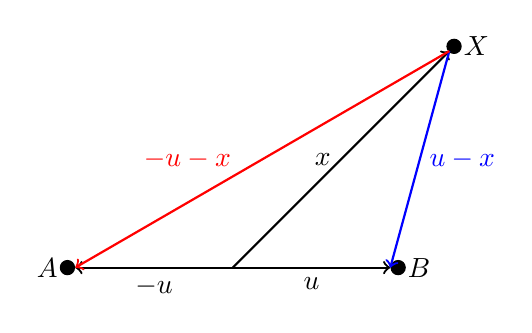
\begin{tikzpicture}
                \draw[thick, ->] (0,0) -- (-2,0);
                \draw[thick, ->] (0,0) -- (2,0);
                
                \draw (-2.1,0) node[anchor=east] {$A$};
                \draw[fill=black] (-2.1,0) circle(0.09);
                
                \draw (2.1,0) node[anchor=west] {$B$};
                \draw[fill=black] (2.1,0) circle(0.09);
                
                \draw (-1,0) node[anchor=north] {$-u$};
                \draw (1,0) node[anchor=north] {$u$};
                
                \draw[thick, ->] (0,0) -- (1.375,1.375) node[anchor=east] {$x$} -- (2.75,2.75);
                
                \draw (2.81,2.81) node[anchor=west] {$X$};
                \draw[fill=black] (2.81,2.81) circle(0.09);
                
                \draw[thick,color=blue,->] (2.75,2.75) -- (2,0);
                \draw[thick,color=red,->] (2.75,2.75) -- (-2,0);
                
                \draw[color=blue] (2.375,1.375) node[anchor=west] {$u-x$};
                \draw[color=red] (0.1,1.375) node[anchor=east] {$-u-x$};
            \end{tikzpicture}
        \end{center}
        
        So that
        \[ \cos{\theta} = \frac{(u-x) \cdot (-u-x)}{\lVert u-x \rVert \lVert u+x \rVert} = \frac{\lVert x \rVert^2 - \lVert u \rVert^2}{\lVert u-x \rVert \lVert u+x \rVert} \]
        
        which defines our locus.
    \end{proof}
\end{exercise} %e1.2.14

\begin{exercise} \label{e1.2.15}
    \begin{enumerate}
        \item Let $y \in \mathbb{R}^n$. If $x \cdot y = 0$ for \emph{all} $x \in \mathbb{R}^n$, then prove that $y=0$.
        
        \item Suppose $y,z \in \mathbb{R}^n$ and $x \cdot y = x \cdot z$ for all $x \in \mathbb{R}^n$. what can you conclude?
    \end{enumerate}
    
    \begin{proof}
        \begin{enumerate}
            \item So $y \cdot y=0$. So
            $$ \sum_{i=1}^n y_i^2 = 0 $$
            if and only if $ y_i=0$ for all $i$.
            
            \item For all $x \in \mathbb{R}^n$ we have
            \begin{align*}
                x \cdot y &= x \cdot z \\
                x \cdot (y-z) &= 0 \\
                \intertext{and so, by the previous,}
                y-z &= 0 \\
                y&=z
            \end{align*}
        \end{enumerate}
    \end{proof}
\end{exercise} %e1.2.15

\begin{exercise} \label{e1.2.16}
    If $x = \begin{bmatrix} x_1 \\ x_2 \end{bmatrix} \in \mathbb{R}^2$, set $\rho(x) = \begin{bmatrix} -x_2 \\ x_1 \end{bmatrix}$.
    
    \begin{enumerate}
        \item Check that $\rho(x)$ is orthogonal to $x$; indeed, $\rho(x)$ is obtained by rotating $x$ an angle $\frac{\pi}{2}$ counterclockwise.
        
        \item Given $x,y \in \mathbb{R}^2$, prove that $x \cdot \rho(y)=-\rho(x) \cdot y$. Interpret this statement geometrically.
    \end{enumerate}
    
    \begin{proof}
        \begin{enumerate}
            \item Observe
            \begin{align*}
                x \cdot \rho(x) &= \begin{bmatrix} x_1 \\ x_2 \end{bmatrix} \cdot \begin{bmatrix} -x_2 \\ x_1 \end{bmatrix} \\
                &= -x_1x_2 + x_1x_2 \\
                &= 0
            \end{align*}
            Thus $x$ and $\rho(x)$ are orthogonal. Now, wlog, let $\vert \vert x \vert \vert = 1$ and let $\theta$ denote the angle between $e_1$ and $x$ opening counter-clockwise. Then 
            $$ x = (x_1,x_2) = (\cos(\theta),\sin(\theta)) $$
            Rotating $x$ counter-clockwise by $\frac{\pi}{2}$, we obtain
            \begin{align*}
                \left( \cos\left( \theta + \frac{\pi}{2} \right), \sin\left( \theta + \frac{\pi}{2} \right) \right) &= (-\sin(\theta),\cos(\theta)) \\
                &= (-x_2,x_1) \\
                &= \rho(x)
            \end{align*}
            
            \item Observe
            $$ x \cdot \rho(y) = -x_1y_2 + x_2y_1 $$
            and
            $$ -\rho(x) \cdot y = x_2y_1 - x_1y_2 $$
            Geometrically, this equality tells us that the angle between $x$ and $\rho(y)$ is equal to the angle between $-\rho(x)$ and $y$.
            \begin{center}
                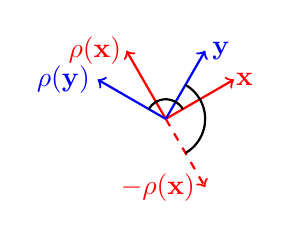
\begin{tikzpicture}
                    \draw[->,thick,red] (0,0) -- (0.866,0.5);
                    \node[red] at (1,0.5) {$\mathbf{x}$};
                    
                    \draw[->,thick,red] (0,0) -- (-0.5,0.866);
                    \node[red] at (-0.9,0.866) {$\mathbf{\rho(x)}$};
                    
                    \draw[->,thick,red,dashed] (0,0) -- (0.5,-0.866);
                    \node[red] at (-0.1,-0.866) {$\mathbf{-\rho(x)}$};
                    
                    \draw[->,thick,blue] (0,0) -- (0.5,0.866);
                    \node[blue] at (0.7,0.866) {$\mathbf{y}$};
                    
                    \draw[->,thick,blue] (0,0) -- (-0.866,0.5);
                    \node[blue] at (-1.3,0.5) {$\mathbf{\rho(y)}$};
                    
                    \draw[black,thick] (0.25,-0.433) arc (-60:60:0.5);
                    
                    \draw[black,thick] (0.2165,0.125) arc (30:150:0.25);
                \end{tikzpicture}
            \end{center}
        \end{enumerate}
    \end{proof}
\end{exercise} %e1.2.16

\begin{exercise} \label{e1.2.17}
    Prove that for any vectors $x,y \in \mathbb{R}^n$, we have $\vert\vert x \vert \vert - \vert \vert y \vert \vert \leq \vert \vert x - y \vert \vert$. Deduce that $\left| \vert \vert x \vert \vert - \vert \vert y \vert \vert \right| \leq \vert \vert x - y \vert \vert$.
    
    \begin{proof}
        Notice
        $$ \vert \vert x \vert \vert = \vert \vert x -y+y \vert \vert \leq \vert \vert x-y \vert \vert + \vert \vert y \vert \vert $$
        which implies the first result. Similarly,
        $$ \vert \vert y \vert \vert = \vert \vert x-y-x \vert \vert \leq \vert \vert x-y \vert \vert + \vert \vert x \vert \vert $$
        So that
        \begin{align*}
            \vert\vert y \vert\vert - \vert\vert x \vert\vert &\leq \vert\vert x - y \vert\vert \\
            \vert\vert x \vert \vert - \vert \vert y \vert \vert &\geq -\vert \vert x - y \vert \vert
        \end{align*}
        which, together with the first result, implies 
        $$ -\vert \vert x - y \vert \vert \leq  \vert\vert x \vert \vert - \vert \vert y \vert \vert \leq \vert \vert x - y \vert \vert$$
        which implies the second result.
    \end{proof}
\end{exercise} %e1.2.17

\begin{exercise} \label{e1.2.18}
    
\end{exercise} %e1.2.18

\begin{exercise} \label{e1.2.19}
    
\end{exercise} %e1.2.19

\begin{exercise} \label{e1.2.20}
    \begin{enumerate}
        \item Let $x$ and $y$ be vector with $\vert\vert x \vert\vert = \vert\vert y \vert\vert$. Prove that the vector $x+y$ bisects the angle between $x$ and $y$.
        
        \item More generally, if $x$ and $y$ are arbitrary nonzero vectors, let $a = \vert\vert x \vert\vert$ and $b=\vert\vert y \vert\vert$. Prove that the vector $bx+ay$ bisects the angle between $x$ and $y$.
    \end{enumerate}
    
    \begin{proof}
        \begin{enumerate}
            \item It is enough to show that $\cos\left( \theta_{x,x+y} \right) = \cos\left( \theta_{y,x+y} \right)$. To that end, 
            $$ x \cdot x = \vert\vert x \vert\vert^2 = \vert\vert y \vert\vert^2 = y \cdot y $$
            Thus 
            \begin{align*} 
                \cos\left( \theta_{x,x+y} \right) &= \frac{x \cdot (x+y)}{\vert\vert x \vert\vert \vert\vert x+y \vert\vert} \\
                &= \frac{(x \cdot x) + (x \cdot y)}{\vert\vert x \vert\vert \vert\vert x+y \vert\vert} \\
                &= \frac{(y \cdot y)+(x \cdot y)}{\vert\vert y \vert\vert \vert\vert x+y \vert\vert} \\
                &= \frac{y \cdot (x+y)}{\vert\vert y \vert\vert \vert\vert x+y \vert\vert} \\
                &=  \cos\left( \theta_{y,x+y} \right) 
            \end{align*}
            
            \item Note then that 
            $$ \vert\vert bx \vert \vert = ab = \vert\vert ay \vert\vert $$
            so that by the previous, the result follows.
        \end{enumerate}
    \end{proof}
\end{exercise} %e1.2.20

\subsection{Subspaces of $\mathbb{R}^n$}
\begin{exercise} \label{e1.3.1}
    trivial
\end{exercise} %e1.3.1

\begin{exercise} \label{e1.3.2}
    trivial
\end{exercise} %e1.3.2

\begin{exercise} \label{e1.3.3}
    Suppose \(x,v_1,\ldots,v_k \in \mathbb{R}^n\) and \(x\) is orthogonal to each of the vectors \(v_1,\ldots,v_k\). Prove that \(x\) is orthogonal to any linear combination \(c_1v_1+c_2v_2+\ldots+c_kv_k\).
    
    \begin{proof}
        \[x \cdot \sum_{i=1}^{k} c_iv_i = \sum_{i=1}^k c_i (x \cdot v_i) = 0\]
    \end{proof}
\end{exercise} %e1.3.3

\begin{exercise} \label{e1.3.4}
    \(V^{\perp}\) is a subspace.
    
    \begin{proof}
        Let \(V\) be a subspace of \( \mathbb{R}^n \). Let \(v \in V \) and \( w \in V^{\perp} \).
        \begin{enumerate}
            \item \(0 \cdot v = 0\), \(\forall v \in V\)
            \item \((w_1+w_2)\cdot v = (w_1,v)+(w_2,v) = 0+0 = 0\)
            \item \(cw \cdot v = c(w \cdot v) = 0\)
        \end{enumerate}
    \end{proof}
\end{exercise} %e1.3.4

\begin{exercise} \label{e1.3.5}
    Given vectors \(v_1,\ldots,v_k \in \mathbb{R}^n\), prove that \(V=\text{Span}(v_1,\ldots,v_k)\) is the \emph{smallest} subspace containing them all. That is, prove that if \(W \subset \mathbb{R}^n\) is a subspace and \(v_1,\ldots,v_k \in W\), then \(V \subset W\).
    
    \begin{proof}
        Note if \(v_1,\ldots,v_k \in W\) then \(\sum \alpha_i v_i \in W\). Thus \(\displaystyle \forall_{v \in V} v \in W\).
    \end{proof}
\end{exercise} %e1.3.5

\begin{exercise} \label{e1.3.6}
    \begin{enumerate}
        \item Let \(U\) and \(V\) be subspaces of \(\mathbb{R}^n\). Define
        \[U \cap V=\{x \in \mathbb{R}^n:x \in U \text{ and } x \in V\}\]
        Prove that \(U\cap V\) is a subspace of \(\mathbb{R}^n\).
        
        \item Is \(U \cup V = \{x \in \mathbb{R}^n:x \in U \text{ or } x \in V\}\) a subspace of \(\mathbb{R}^n\)? Give a proof or counterexample.
        
        \item Let \(U\) and \(V\) be subspaces of \(\mathbb{R}^n\). Define
        \[U+V=\{x \in \mathbb{R}^n: x=u+v \text{ for some } u\in U \text{ and } v\in V\}\]
        Prove that \(U+V\) is a subspace of \(\mathbb{R}^n\).
        
    \end{enumerate}
    
    \begin{proof}
        \begin{enumerate}
            \item
                \begin{enumerate}
                    \item \(0\in U \cap V\)
                    
                    \item If \(y,x\in U\cap V\) then \(x+y\in U \cap V\)
                    
                    \item \(\forall_{x\in U \cap V} cx \in U \cap V\)
                \end{enumerate}
            
            \item No. Let \(U=\text{Span}\begin{bmatrix}1 \\ 0\end{bmatrix}\), \(V=\text{Span}\begin{bmatrix}0 \\ 1\end{bmatrix}\) then \(\begin{bmatrix}1 \\ 1\end{bmatrix} \not\in U \cup V\)
            
            \item 
                \begin{enumerate}
                    \item \(0=0+0\)
                    
                    \item \(x_1+x_2=u_1+v_1+u_2+v_2=(u_1+u_2)+(v_1+v_2)\)
                    
                    \item \(cx=c(u_1+v)=cu+cv\)
                \end{enumerate}
        \end{enumerate}
    \end{proof}
\end{exercise} %e1.3.6

\begin{exercise} \label{e1.3.7}
    Let \(v_1,\ldots,v_k \in \mathbb{R}^n\) and let \(v \in \mathbb{R}^n\). Prove that
    \[\text{Span}(v_1,\ldots,v_k)=\text{Span}(v_1,\ldots,v_k,v) \iff v \in \text{Span}(v_1,\ldots,v_k)\]
    
    \begin{proof}
        Let \(v \in \text{Span}(v_1,\ldots,v_k)\) then
        \[v=\sum \alpha_i v_i\]
        Clearly \(\text{Span}(v_1,\ldots,v_k) \subset \text{Span}(v_1,\ldots,v_k,v)\). Now if \(u\in \text{Span}(v_1,\ldots,v_k,v)\) then
        \begin{align*}
            u &= \sum_{i=1}^k \beta_i v_i + \beta_{k+1}v \\
            &= \sum \beta_i v_i + \beta_{k+1}(\sum \alpha_i v_i)
        \end{align*}
        
        Now let \(\text{Span}(v_1,\ldots,v_k)=\text{Span}(v_1,\ldots,v_k,v)\). Then
        \begin{align*}
            \sum_{i=1}^k \alpha_i v_i + v &= \sum \beta_i v_i \\
            v &= \sum_{i=1}^k (\beta_i-\alpha_i)v_i
        \end{align*}
    \end{proof}
\end{exercise} %e1.3.7

\begin{exercise} \label{e1.3.8}
    Let \(V \subset \mathbb{R}^n\) be a subspace. Prove that \(V \cap V^{\perp}=\{0\}\).
    
    \begin{proof}
        Recall that \(x \cdot x = 0\) iff \(x=0\). Note \(V \cap V^{\perp} \subset V, V^{\perp}\). Clearly \( 0 \in V \cap V^\perp \). So \( x \in V \cap V^{\perp}\) iff \( \forall_{v \in V} v \cdot x = 0 \) and \(x \in V\) iff \(x \cdot x = 0\) iff \(x=0\). Thus \(V \cap V^{\perp}=\{0\}\).
    \end{proof}
\end{exercise} %e1.3.8

\begin{exercise} \label{e1.3.9}
    Suppose \(U,V \subset \mathbb{R}^n\) are subspaces and \(U \subset V\). Prove that \(V^{\perp} \subset U^{\perp}\).
    
    \begin{proof}
        Let \(U \subset V\) and let \(v'\in V^{\perp}\). So \(\forall_{v \in V} v' \cdot v=0\). Thus \(\forall_{u \in U} v' \cdot u=0\). Thus \(v' \in U^{\perp}\).
    \end{proof}
\end{exercise} %e1.3.9

\begin{exercise} \label{e1.3.10}
    Let \(V \subset \mathbb{R}^n\) be a subspace. Prove that \(V \subset \left(V^{\perp}\right)^{\perp}\). Do you think more is true?
    
    \begin{proof}
        \[x \in \left(V^{\perp}\right)^{\perp} \text{ iff } \forall_{v' \in V^{\perp}} x \cdot v' = 0 \text{ iff } x \in V\]
    \end{proof}
\end{exercise} %e1.3.10

\subsection{Linear Transformations and Matrix Algebra}

\begin{exercise} \label{e1.4.1}
    Trivial
\end{exercise} %e1.4.1

\begin{exercise} \label{e1.4.2}
    \begin{enumerate}
        \item If \(A\) is an \(m \times n\) matrix and \(Ax=0\) for all \(x \in \mathbb{R}^n\), prove that \(A=0\). 
        
        \item If \(A\) and \(B\) are \(m \times n\) matrices and \(Ax=Bx\) for all \(x \in \mathbb{R}^n\), prove that \(A=B\).
    \end{enumerate}
    
    \begin{proof}
        \begin{enumerate}
            \item We proceed by contrapositive and suppose \(A\neq 0\). Then there is \(i,j\) such that \([A]_{ij}\neq 0\). Let \(x=A_{i}^{T}\), where \( A_{i}^{T}\) is the \(i^{\text{th}}\) row of \(A\). Then
            \[[Ax]_{i,1}=x \cdot x>0\]
            so that there exists x such that \(Ax \neq 0 \).
            \item For all \( x \) we have
            \begin{align*}
                Ax &= Bx \\
                (A-B)x &= 0
            \end{align*}
            so by the previous, \(A-B=0\). So \(A=B\).
        \end{enumerate}
    \end{proof}
\end{exercise} %e1.4.2

\begin{exercise} \label{e1.4.3}
    Let \( A \) be an \(m \times n\) matrix. Show that \(V = \{x \in \mathbb{R}^n : Ax=0 \}\) is a subspace of \(\mathbb{R}^n\).
    
    \begin{proof}
        Let \(x,y \in v\). So
        \[ A(\alpha x+\beta y) = \alpha Ax + \beta Ay = 0 \]
        So \(\alpha x + \beta y \in V\). Thus, by the subspace Lemma, \(V\) is a subspace of \(\mathbb{R}^n\).
    \end{proof}
\end{exercise} %e1.4.3

\begin{exercise} \label{e1.4.4}
    Let \( A \) be an \(m \times n\) matrix.
    \begin{enumerate}
        \item Show that \(\left\{ \begin{bmatrix} x \\ Ax \end{bmatrix} : x \in \mathbb{R}^n \right\}\) is a subspace of \(\mathbb{R}^{n+m}\).
        
        \item When \(m=1\) show that \(V \subset \mathbb{R}^{n+1}\) is a hyperplane by finding a vector \(b \in \mathbb{R}^{n+1}\) so that \( V=\{ z \in \mathbb{R}^{n+1} : b \cdot z = 0 \} \).
    \end{enumerate}
    
    \begin{proof}
        \begin{enumerate}
            \item Let \( \begin{bmatrix} x \\ Ax \end{bmatrix}, \begin{bmatrix} y \\ Ay \end{bmatrix} \in V \). So
            \begin{align*}
                \alpha \begin{bmatrix} x \\ Ax \end{bmatrix} + \beta \begin{bmatrix} y \\ Ay \end{bmatrix} &= \begin{bmatrix} \alpha x + \beta y \\ \alpha Ax + \beta Ay \end{bmatrix} \\
                &= \begin{bmatrix} \alpha x + \beta y \\ A\alpha x +  A \beta y \end{bmatrix} \\
                &= \begin{bmatrix} \alpha x + \beta y \\ A(\alpha x + \beta y) \end{bmatrix} \in V
            \end{align*}
            Thus, by the Subspace Lemma, \(V\) is a subspace of \(\mathbb{R}^{n+m}\).
            
            \item Notice
            \begin{align*}
                \begin{bmatrix} -A_1^T \\ 1 \end{bmatrix} \cdot \begin{bmatrix} x \\ Ax \end{bmatrix} &= (-A_1)^T \cdot x + Ax \\
                &= -(A_1)^T \cdot x + A_1^T \cdot x \\
                &= 0
            \end{align*}
            where \(A_1\) is the first row of the matrix \(A\).
        \end{enumerate}
    \end{proof}
\end{exercise} %e1.4.4

\begin{exercise} \label{e1.4.5}
    Give \( 2 \times 2 \) matrices \( A \) so that for any \( x \in \mathbb{R}^2 \) we have, respectively,
    \begin{enumerate}
        \item \( Ax \) is the vector whose components are, respectively, the sum and difference of the components of \( x \);
        
        \item \( Ax \) is the vector obtained by projecting \( x \) onto the line \( x_1 = x_2 \) in \( \mathbb{R}^2 \);
        
        \item \( Ax \) is the vector obtained by first reflecting \( x \) across the line \( x_1 = 0 \) and then reflecting the resulting vector across the line \( x_2 = 0 \);
        
        \item \( Ax \) is the vector obtained by projecting \( x \) onto the line \( 2x_1-x_2=0\);
        
        \item \( Ax \) is the vector obtained by first projecting \( x \) onto the line \( 2x_1-x_2=0 \) and then rotating the resulting vector \( \frac{\pi}{2} \) counterclockwise;
        
        \item \( Ax \) is the vector obtained by first rotating \( x \) an angle of \( \frac{\pi}{2} \) counterclockwise and then projecting the resulting vector onto the line \( 2x_1-x_2=0 \).
    \end{enumerate}
    
    \begin{proof}
        \begin{enumerate}
            \item \( A = \begin{bmatrix} 1 & 1 \\ 1 & -1 \end{bmatrix} \)
            
            \item \( A = \begin{bmatrix} \frac{1}{2} & \frac{1}{2} \\ & \\ \frac{1}{2} & \frac{1}{2} \end{bmatrix} \)
            
            \item \( A = \begin{bmatrix} -1 & 0 \\ 0 & -1 \end{bmatrix} \)
            
            \item \( A = \begin{bmatrix} \frac{1}{5} & \frac{2}{5} \\ & \\ \frac{2}{5} & \frac{4}{5} \end{bmatrix} \)
            
            \item \( A = \begin{bmatrix} 0 & -1 \\ 1 & 0 \end{bmatrix} \begin{bmatrix} \frac{1}{5} & \frac{2}{5} \\ & \\ \frac{2}{5} & \frac{4}{5} \end{bmatrix} = \begin{bmatrix} -\frac{2}{5} & -\frac{4}{5} \\ \frac{1}{5} & \frac{2}{5} \end{bmatrix} \)
            
            \item Reverse the order of multiplication in the previous.
        \end{enumerate}    
    \end{proof}
\end{exercise} %e1.4.5

\begin{exercise} \label{e1.4.6}

\end{exercise} %e1.4.6

\begin{exercise} \label{e1.4.7}
    Let \( A_\theta \) be the rotation matrix, \( 0 \leq \theta \leq \pi \). Prove
    
    \begin{enumerate}
        \item \( \vert\vert A_\theta x \vert \vert = \vert\vert x \vert\vert \) for all \( x \in \mathbb{R}^2 \)
        
        \item the angle between \( x \) and \( A_\theta x \) is \( \theta \).
    \end{enumerate}
    
    \begin{proof}
        \begin{enumerate}
            \item \begin{align*}
                \vert\vert A_\theta x \vert \vert^2 &= \left|\left| \begin{bmatrix} \cos(\theta)x_1 - \sin(\theta)x_2 \\ sin(\theta)x_1+\cos(\theta)x_2 \end{bmatrix} \right|\right|^2 \\
                &= \left( \cos(\theta)x_1 - \sin(\theta)x_2 \right)^2 + \left( \sin(\theta)x_1+\cos(\theta)x_2 \right)^2 \\
                &= x_1^2(\sin^2(\theta)+\cos^2(\theta))+x_2^2(\sin^2(\theta)+\cos^2(\theta)) \\
                &= x_1^2+x_2^2 \\
                &= \left|\left| x \right|\right|^2
            \end{align*}
            
            \item \begin{align*}
                A_\theta x \cdot x &= \begin{bmatrix} \cos(\theta)x_1 - \sin(\theta)x_2 \\ sin(\theta)x_1+\cos(\theta)x_2 \end{bmatrix} \cdot \begin{bmatrix} x_1 \\ x_2 \end{bmatrix} \\
                &= \cos(\theta)x_1^2-\sin(\theta)x_1x_2+\sin(\theta)x_1x_2+\cos(\theta)x_2^2 \\
                &= \cos(\theta)\left|\left| x \right|\right|^2
            \end{align*}
            which implies the result.
        \end{enumerate}
    \end{proof}
\end{exercise} %e1.4.7

\begin{exercise} \label{e1.4.8}
    Prove or give a counterexample. Assume all relevant matrices are square and of the same size.
    
    \begin{enumerate}
        \item If \( AB = CB \) and \( B \neq 0 \), then \( A = C \).
        
        \item If \( A^2 = A \), then \( A = 0 \) or \( A = I \).
        
        \item \( (A+B)(A-B) = A^2 - B^2 \).
        
        \item If \( AB = BC \) and \( B \) is invertible, then \( A = C \).
    \end{enumerate}
    
    \begin{proof}
        \begin{enumerate}
            \item Let
            \begin{align*}
                A &= 0 \\
                B &= \begin{bmatrix} 1 & 0 \\ 0 & 0 \end{bmatrix} \\
                C &= \begin{bmatrix} 0 & 1 \\ 0 & 0 \end{bmatrix} \\
            \end{align*}
            Then 
            \[ AB = 0 = CB \]
            but \( A \neq C \) and \( B \neq 0 \).
            
            \item Let \( A = \begin{bmatrix} 0 & 1 \\ 0 & 1 \end{bmatrix} \). Then \( A^2 = A \) but \( A \neq I,0 \).
            
            \item Let \( A = \begin{bmatrix} 1 & 0 \\ 0 & 0 \end{bmatrix} \) and \( B = \begin{bmatrix} 1 & 1 \\ 0 & 0 \end{bmatrix} \). Then
            \begin{align*}
                (A-B)(A+B) &= 0 \\
                A^2 - B^2 &= \begin{bmatrix} 0 & -1 \\ 0 & 0 \end{bmatrix}
            \end{align*}
            
            \item Let
            \begin{align*}
                A &= \begin{bmatrix} 1 & 0 \\ 0 & 0 \end{bmatrix} \\
                B &= \begin{bmatrix} 1 & 1 \\ 0 & 1 \end{bmatrix} \\
                C &= \begin{bmatrix} 1 & 1 \\ 0 & 0 \end{bmatrix}
            \end{align*}
            Then \( AB = C = BC \) and \( A \neq C \) and \( B \) is invertible.
        \end{enumerate}
    \end{proof}
\end{exercise} %e1.4.8

\begin{exercise} \label{e1.4.9}
    Fin all \( 2 \times 2 \) matrices \( A = \begin{bmatrix} a & b \\ c & d \end{bmatrix} \) satisfying
    
    \begin{enumerate}
        \item \( A^2 = I_2 \)
        \item \( A^2 = 0 \)
        \item \( A^2 = -I_2 \)
    \end{enumerate}
    
    \begin{proof}
        %proof here
    \end{proof}
\end{exercise} %e1.4.9

\begin{exercise} \label{e1.4.10}
    %
\end{exercise} %e1.4.10

\begin{exercise} \label{e1.4.11}
    For each of the following matrices \( A \), find a formula for \( A^n \). (If you know how to give an inductive proof, please do so.)
    
    \begin{enumerate}
        \item \( A = \begin{bmatrix} 1 & 1 \\ 0 & 1 \end{bmatrix} \)
        \item \( A = \begin{bmatrix} d_1 & & & \\ & d_2 & & \\ & & \ddots & \\ & & & d_m \end{bmatrix} \)
    \end{enumerate}
    
    \begin{proof}
        \begin{enumerate}
            \item We claim \( A^n = \begin{bmatrix} 1 & n \\ 0 & 1 \end{bmatrix} \). It's simple to verify that \( A^2 = \begin{bmatrix} 1 & 2 \\ 0 & 1 \end{bmatrix} \). Now, suppose the claim holds for \( n \). Then 
            
            \[
                A^n A = \begin{bmatrix} 1 & n \\ 0 & 1 \end{bmatrix} \begin{bmatrix} 1 & 1 \\ 0 & 1 \end{bmatrix} = \begin{bmatrix} 1 & n+1 \\ 0 & 1 \end{bmatrix} = A^{n+1}
            \]
            
            \item We claim \( A^n = \begin{bmatrix} d_1^n & & & \\ & d_2^n & & \\ & & \ddots & \\ & & & d_m^n \end{bmatrix} \). This is simple to verify for \( n = 2 \). Now suppose the claim holds for \( n \). Then
            \[
                A^{n+1} = A^n A = \begin{bmatrix} d_1^n & & & \\ & d_2^n & & \\ & & \ddots & \\ & & & d_m^n \end{bmatrix} \begin{bmatrix} d_1 & & & \\ & d_2 & & \\ & & \ddots & \\ & & & d_m \end{bmatrix} = \begin{bmatrix} d_1^{n+1} & & & \\ & d_2^{n+1} & & \\ & & \ddots & \\ & & & d_m^{n+1} \end{bmatrix} 
            \]
        \end{enumerate}
    \end{proof}
\end{exercise} %e1.4.11

\begin{exercise} \label{e1.4.12}
    %
\end{exercise} %e1.4.12

\begin{exercise} \label{e1.4.13}
    %
\end{exercise} %e1.4.13

\begin{exercise} \label{e1.4.14}
    %
\end{exercise} %e1.4.14

\begin{exercise} \label{e1.4.15}
    %
\end{exercise} %e1.4.15

\begin{exercise} \label{e1.4.16}
    %
\end{exercise} %e1.4.16

\begin{exercise} \label{e1.4.17}
    %
\end{exercise} %e1.4.17

\begin{exercise} \label{e1.4.18}
    Find matrices \( A \) so that
    \begin{enumerate}
        \item \( A \neq 0 \), but \( A^2 = 0 \)
        \item \( A^2 \neq 0 \) , but \( A^3 = 0 \)
    \end{enumerate}
    
    \begin{proof}
        \begin{enumerate}
            \item \( \begin{bmatrix} 0 & 1 \\ 0 & 0 \end{bmatrix} \)
            
            \item \( \begin{bmatrix} 0 & 1 & 1 \\ 0 & 0 & 1 \\ 0 & 0 & 0 \end{bmatrix} \)
        \end{enumerate}
    \end{proof}
\end{exercise} %e1.4.18

\begin{exercise} \label{e1.4.19}
    Suppose \( A \) is an invertible \( n \times n \) matrix and \( x \in \mathbb{R}^n \) satisfies \( Ax = 7x \). Calculate \( A^{-1}x \).
    
    \begin{proof}
        We know \( A^{-1}A = I_n \). Thus 
        \[ A^{-1}Ax = 7A^{-1}x = x \]
        implying \( A^{-1}x = \frac{1}{7}x \)
    \end{proof}
\end{exercise} %e1.4.19

\begin{exercise} \label{e1.4.20}
    Suppose \( A \) is a square matrix satisfying the equation \( A^3 - 3A + 2I = 0 \). Show that \( A \) is invertible.
    
    \begin{proof}
        \begin{align*}
            A^3 - 3A + 2I &= 0 \\
            A^3 - 3A &= -2I \\
            A(A^2 - 3I) &= -2I \\
            \frac{1}{2}A(A^2 - 3I) &= I
        \end{align*}
        implying \( A^{-1} = \frac{1}{2}(A^2 - 3I) \)
    \end{proof}
\end{exercise} %e1.4.20

\begin{exercise} \label{e1.4.21}
    Suppose \( A \) is an \( n \times n \) matrix satisfying \( A^{10} = 0 \). Prove that the matrix \( I_n - A \) is invertible.
    
    \begin{proof}
        \[ (I_n - A)(I_n^9 + I_n^8A + \ldots + I_nA^8 + A^9) = I_n^{10} - A^{10} = I_n - A^{10} = I_n  \]
        implying \( I_n - A \) is invertible.
    \end{proof}
\end{exercise} %e1.4.21

\begin{exercise} \label{e1.4.22}
    Define the \emph{trace} of an \( n \times n \) matrix \( A \) (denoted \( trA \)) to be the sum of its diagonal entries:
    \[ trA = \sum_{i=1}^{n}a_{ii} \]
    
    \begin{enumerate}
        \item Prove that \( trA = trA^T \)
        \item Prove that \( tr(A+B) = trA + trB \) and \( trcA = ctrA\)
        \item Prove that \( trAB = trBA \)
    \end{enumerate}
    
    \begin{proof}
        \begin{enumerate}
            \item 
            \[ trA^T = \sum_{i=1}^n \left[ A^T \right]_{ii} = \sum_{i=1}^n \left[ A \right]_{ii} = trA \]
            
            \item Trivial
            
            \item
                \begin{align*}
                    trAB &= \sum_{i=1}^n \left[ AB \right]_{ii} \\
                    &= \sum_{i=1}^n \left( \sum_{r=1}^n [A]_{ir}[B]_{ri} \right) \\
                    &= \sum_{i=1}^n\sum_{r=1}^n [A]_{ir}[B]_{ri} \\
                    &= \sum_{r=1}^n\sum_{i=1}^n [A]_{ir}[B]_{ri} \\
                    &= \sum_{r=1}^n\sum_{i=1}^n [B]_{ri}[A]_{ir} \\
                    &= \sum_{r=1}^n [BA]_{ii} \\
                    &= trBA
                \end{align*}
        \end{enumerate}
    \end{proof}
\end{exercise} %e1.4.22

\begin{exercise} \label{e.1.4.23}
    %
\end{exercise} %e1.4.23

\begin{exercise} \label{e1.4.24}
    Suppose \( A \) and \( B \) are symmetric. Prove that \( AB \) is symmetric if and only if \( AB = BA \).
    
    \begin{proof}
        If \( AB \) is symmetric then
        \[ AB = (AB^T) = B^TA^T = BA \]
        If \( AB = BA \) then
        \[ (AB)^T = B^TA^T = BA = AB \]
    \end{proof}
\end{exercise} %e1.4.24

\begin{exercise} \label{e1.4.25}
    Let \( A \) be an arbitrary \( m \times n \) matrix. Prove that \( A^TA \) is symmetric.
    
    \begin{proof}
        \[ (A^TA) = A^T(A^T)^T = A^TA \]
    \end{proof}
\end{exercise} %e1.4.25

\begin{exercise} \label{e1.4.26}
    %
\end{exercise} %e1.4.26

\begin{exercise} \label{e1.4.27}
    %
\end{exercise} %e1.4.27

\begin{exercise} \label{e1.4.28}
    An \( n \times n \) matrix is called a \emph{permutation matrix} if it has a single 1 in each row and column and all its remaining entries are \( 0 \).
    
    \begin{enumerate}
        \item Write down all the \( 2 \times 2 \) permutation matrices. How many are there?
        
        \item Write down all the \( 3 \times 3 \) permutation matrices. How many are there?
        
        \item Prove that the product of two permutation matrices is again a permutation matrix. Do they commute?
    \end{enumerate}
    
    \begin{proof}
        \begin{enumerate}
            \item 
            
            \item
            
            \item
        \end{enumerate}
    \end{proof}
\end{exercise} %e1.4.28

\begin{exercise} \label{e1.4.29}
    Let \( A \) be an \( m \times n \) matrix and let \( x,y \in \mathbb{R}^n \). Prove that if \( Ax = 0 \) and \( y = A^Tb \) for some \( b \in \mathbb{R}^m \) then \( x \cdot y = 0 \).
    
    \begin{proof}
        \begin{align*}
            x \cdot y &= y^Tx \\
            &= \left( b^TA \right)x \\
            &= b^T\left(Ax\right) \\
            &= b^T 0 \\
            &= 0
        \end{align*}
    \end{proof}
\end{exercise} %e.1.4.29

\begin{exercise} \label{e1.4.30}
    %
\end{exercise} %e1.4.30

\begin{exercise} \label{e1.4.31}
    %
\end{exercise} %e1.4.31

\begin{exercise} \label{e1.4.32}
    Suppose \( A \) is an \( m \times n \) matrix and \( x \in \mathbb{R}^n \) satisfies \( (A^TA)x = 0 \). Prove that \( Ax = 0 \).
    
    \begin{proof}
        Note that \( A^TAx = 0 \) implies
        \begin{align*}
            0 &= A^TAx \cdot x \\
            &= x \cdot (A^TA)^Tx \\
            \intertext{and by symmetry of \( A^TA \) }
            &= x \cdot A^TAx \\
            &= x^TA^TAx \\
            &= (Ax)^T(Ax) \\
            &= \vert \vert Ax \vert \vert^2
        \end{align*}
        implying \( Ax = 0 \)
    \end{proof}
\end{exercise} %e1.4.32

\begin{exercise} \label{e1.4.33}
    Suppose \( A \) is a symmetric matrix satisfying \( A^2 = 0 \). Prove that \( A = 0 \). Give an example to show that the hypothesis of symmetry is required.
    
    \begin{proof}
        Since \( A \) is symmetric, we have \( A^T = A \) and \( 0 = A^2 = A^TA \). Thus, by \ref{e1.4.32}
        \begin{align*}
            A^TA &= 0 \hspace{2mm} \forall x \\
            \intertext{ implies }
            Ax &= 0 \hspace{2mm} \forall x \\
            \intertext{ implies }
            A &= 0
        \end{align*}
    \end{proof}
\end{exercise} %e1.4.33

\begin{exercise} \label{e1.4.34}
    We say an \( n \times n \) matrix \( A \) is \emph{orthogonal} if \( A^TA = I_n \).
    
    \begin{enumerate}
        \item Prove that the column vectors \( a_1, \ldots, a_n \) of an orthogonal matrix \( A \) are unit vectors that are orthogonal to one another; i.e.,
        \[ a_i \cdot a_j = \begin{cases} 1, &i=j \\ 0, &i\neq j \end{cases} \]
        
        \item Fill in the missing columns in the following matrices to make them orthogonal:
        \[
            \begin{bmatrix}
                \frac{\sqrt{3}}{2} & ? \\ 
                -\frac{1}{2} & ? 
            \end{bmatrix},
            \begin{bmatrix}
                1 & 0 & ? \\ 
                0 & -1 & ? \\ 
                0 & 0 & ?
            \end{bmatrix},
            \begin{bmatrix}
                \frac{1}{3} & ? & \frac{2}{3} \\
                \frac{2}{3} & ? & -\frac{2}{3} \\
                \frac{2}{3} & ? & \frac{1}{3}
            \end{bmatrix}
        \]
        
        \item Prove that any \( 2 \times 2 \) orthogonal matrix \( A \) must be of the form
        \[
            \begin{bmatrix}
                \cos(\theta) & -\sin(\theta) \\
                \sin(\theta) & \cos(\theta)
            \end{bmatrix}
            \text{ or }
            \begin{bmatrix}
                \cos(\theta) & \sin(\theta) \\
                \sin(\theta) & -\cos(\theta)
            \end{bmatrix}
        \]
        for some real \( \theta \).
        
        \item Prove that if \( A \) is an orthogonal \( 2 \times 2 \) matrix, then \( \mu_A: \mathbb{R}^2 \rightarrow \mathbb{R}^2 \) is either a rotation or the composition of a rotation and a reflection.
        
        \item Assume for now that \( A^T = A^{-1} \) when \( A \) is orthogonal (this is a consequence of a corollary from a future chapter in the book). Prove that the row vectors \( A_1, \ldots, A_n \) of an orthogonal matrix \( A \) are unit vectors that are orthogonal to one another.
    \end{enumerate}
    
    \begin{proof}
        \begin{enumerate}
            \item pending
            
            \item pending
            
            \item pending
            
            \item pending
            
            \item pending
        \end{enumerate}
    \end{proof}
\end{exercise} %e1.4.34

\begin{exercise} \label{e1.4.35}
    Recall the definition of orthogonal matrices from \ref{e1.4.34}
    
    \begin{enumerate}
        \item Prove that if \( A \) and \( B \) are orthogonal \( n \times n \) matrices, then so is \( AB \).
        
        \item Prove that if \( A \) is an orthogonal matrix, then so is \( A^{-1} \)
    \end{enumerate}
    
    \begin{proof}
        \begin{enumerate}
            \item pending
            
            \item pending
        \end{enumerate}
    \end{proof}
\end{exercise} %e1.4.35

\begin{exercise} \label{e1.4.36}
    \begin{enumerate}
        \item Prove that the only matrix that is both symmetric and skew-symmetric is \( 0 \).
        
        \item Given any square matrix \( A \), prove that \( S = \frac{1}{2}(A+A^T) \) is symmetric and \( K = \frac{1}{2}(A-A^T) \) is skew-symmetric.
        
        \item Prove that any square matrix \( A \) can be written in the form \( A = S + K \), where \( S \) is symmetric and \( K \) is skew-symmetric.
        
        \item Prove that the expression in part \( c \) is unique.
    \end{enumerate}
    
    \begin{proof}
        \begin{enumerate}
            \item pending
            
            \item pending
            
            \item pending
            
            \item pending
        \end{enumerate}
    \end{proof}
\end{exercise} %e1.4.36

\begin{exercise} \label{e1.4.37}
    Suppose \( A \) is an \( n \times n \) matrix that commutes with all \( n \times n \) matrices; i.e. \( AB = BA \) for all \( B \in \mathcal{M}_{n \times n} \). What can you say about \( A \)?
    
    \begin{proof}
        pending
    \end{proof}
\end{exercise} %e1.4.37

\subsection{Introduction to Determinants and the Cross Product}